
\xdef\Resistance{2}
\xdef\Inductance{0.005}
\xdef\Period{0.02}
\xdef\IO{-96.4}
\xdef\Vd{200}


\begin{center}
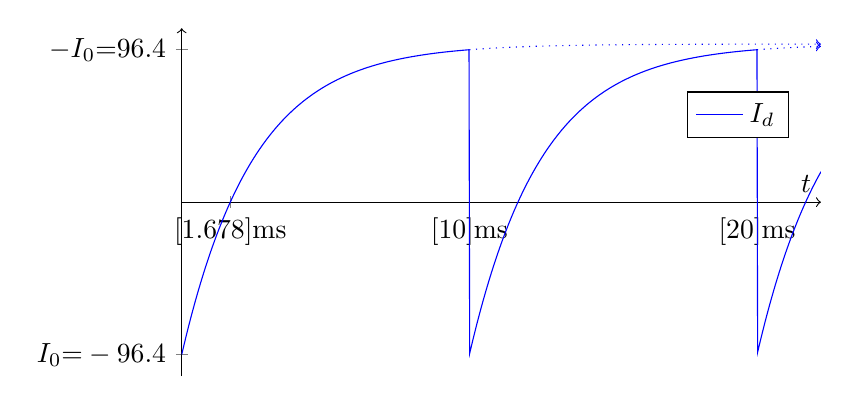
\begin{tikzpicture}
\begin{axis}[domain=0:400, 
             axis x line=middle, 
             axis y line=left, 
             xtick={30.366,180,360}, 
             xticklabels={\unit[1.678]{ms},
                          \unit[10]{ms},
                          \unit[20]{ms},
                          },
             ytick={-96.4,96.4},
             yticklabels={%$-\frac{V_d}{R}{=}-100$,
                          $I_0{=}-96.4$,
                          $-I_0{=}96.4$,
                          %$\frac{V_d}{R}{=}100$},
                          },
             x axis line style={->},
             xlabel={$t$},
             xlabel style={align=right}, 
             y axis line style={->},
             width=0.8\textwidth,
             height=6cm,
             %width=\uncontrolledRectifierGraphWidth,
             ymax=110,
             ymin=-110,
             legend style={at={(axis cs:380,70),anchor=south west}}
             ] 
    \addplot[blue, samples=1000] {
    (
       (\Vd/\Resistance) + (\IO-\Vd/\Resistance) *    exp(-\Resistance*mod(x,180)*\Period/(\Inductance*360))
    )
    }; 
    \addplot[blue, dotted, samples=1000, domain=180:400, ->] {
       (\Vd/\Resistance) + (\IO-\Vd/\Resistance) *    exp(-\Resistance*x*\Period/(\Inductance*360))
    };% 
    \node[right] at (400,100) {to $\frac{V_d}{R}{=}\unit[100]{A}$}; 
    \addplot[blue, dotted, samples=1000, domain=360:400, ->] {(1)*(
       (\Vd/\Resistance) + (\IO-\Vd/\Resistance) *    exp(-\Resistance*(x-180)*\Period/(\Inductance*360))
       )
    };
    \legend{$I_d$}
\end{axis}
\end{tikzpicture}
\end{center}